%% LyX 2.2.0 created this file.  For more info, see http://www.lyx.org/.
%% Do not edit unless you really know what you are doing.
\documentclass[english]{beamer}
\usepackage[T1]{fontenc}
\usepackage[latin9]{inputenc}
\usepackage{amsmath}
\usepackage{amssymb}
\usepackage{graphicx}

\makeatletter
%%%%%%%%%%%%%%%%%%%%%%%%%%%%%% Textclass specific LaTeX commands.
 % this default might be overridden by plain title style
 \newcommand\makebeamertitle{\frame{\maketitle}}%
 % (ERT) argument for the TOC
 \AtBeginDocument{%
   \let\origtableofcontents=\tableofcontents
   \def\tableofcontents{\@ifnextchar[{\origtableofcontents}{\gobbletableofcontents}}
   \def\gobbletableofcontents#1{\origtableofcontents}
 }

%%%%%%%%%%%%%%%%%%%%%%%%%%%%%% User specified LaTeX commands.
\mode<presentation>
{
\usetheme{Moo}
%\usetheme{Pittsburgh}
%\setbeamercovered{transparent = 28}
}

\usepackage{graphicx}
\usepackage{graphics}
\usepackage{hyperref}
\usepackage[english]{babel}

\newenvironment{wideitemize}{\itemize\addtolength{\itemsep}{10pt}}{\enditemize}

%\renewcommand{\section}[1]{\section{#1} \subsection{#1}}
\renewcommand{\makebeamertitle}{\begin{frame}[plain]
\titlepage
\end{frame}}


\usepackage{tikz}
\usetikzlibrary{shadows}
\usetikzlibrary{shadows.blur}
%\usetikzlibrary{shapes.symbols}

\usepackage[T1]{fontenc}
\usepackage{pslatex}

\makeatother

\usepackage{babel}
\begin{document}


\title[Rent-Capture Potential]{Urban Infrastructure Investment and Rent-Capture Potentials }

\subtitle{A case study on Paris urban area}

\author[V. Vigui� (CIRED)]{V.~Vigui�\inst{1} \and S.~Hallegatte\inst{2}}

\institute[...]{\inst{1}CIRED\\
Ecole des Ponts ParisTech, Paris, France\and \inst{2}The World Bank}

\date[]{ FAERE Conference, \today }

\makebeamertitle

\AtBeginSubsection[]{%
  \frame<beamer>{ 
    \frametitle{Outline}   
    \tableofcontents[currentsection,currentsubsection]
  }
}

%\beamerdefaultoverlayspecification{<+->}
\begin{frame}{Outline}

\tableofcontents{}

\end{frame}

\section{Motivation}

\subsection*{} 
\begin{frame}{Make Titles Informative. }


\framesubtitle{}
\begin{itemize}
\item Use Itemize a lot.


\pause{}
\item Use very short sentences or short phrases.


\pause{}
\item These overlays are created using the Pause style.
\end{itemize}

\pause{}
\begin{itemize}
\item It's really easy to write an equation :
\[
\begin{cases}
\frac{\sum_{i=0}^{N}e^{-i.log(i)}}{K}\\
\frac{\partial U}{\partial x}
\end{cases}
\]
 
\end{itemize}
\end{frame}

\begin{frame}[plain]{A \textquotedbl{}plain frame\textquotedbl{}}
\label{plain}

\begin{itemize}
\item In a \textquotedbl{}plain frame\textquotedbl{}, no header and footer
\item This enable to save space, e.g. to put a big graph on the slide
\end{itemize}
\end{frame}
\begin{frame}{Make Titles Informative.}

\begin{block}<1->{}

\begin{itemize}
\item Untitled block.
\item Shown on all slides.
\end{itemize}
\end{block}
\begin{exampleblock}<2->{Some Example Block Title}

\begin{itemize}
\item $e^{i\pi}=-1$.
\item $e^{i\pi/2}=i$.
\end{itemize}
\end{exampleblock}
\end{frame}

\begin{frame}[shrink]{Land value capture}

\begin{itemize}
\item The option \textquotedbl{}shrink\textquotedbl{}enables to put a lot
of text on one slide\medskip{}
\item Efficient public transport systems lie at the core of sustainable
development 

\begin{itemize}
\item However, financing them at a global scale is challenging 
\item Fares do generally not cover full costs 
\end{itemize}

\pause{}
\item Land value capture History: 

\begin{itemize}
\item Henry George (1884) 
\item Successful public transport systems lead to increasing land values,
resulting from the increase in accessibility 
\item Capturing part of land value increase : a promising alternative method
of revenue generation ? 
\end{itemize}

\pause{}
\item In practice 

\begin{itemize}
\item Might be achieved through different policies (land value taxes, land
betterment taxes\dots ) 
\item Bogot�, London, Singapore, Hong Kong, and various cities in Brazil,
Argentina and India 
\item See for instance: Peterson (2009). \emph{Unlocking land values to
finance urban infrastructure} (World Bank Publication) 
\end{itemize}
\end{itemize}
\end{frame}

\begin{frame}{Make Titles Informative. }

\begin{example}<1->
On first slide. 
\end{example}

\begin{example}<2->
On second slide.
\end{example}

\end{frame}

\section{Our Results/Contribution}

\subsection{Main Results}
\begin{frame}{Make Titles Informative. }

\begin{theorem}
On first slide.
\end{theorem}


\pause{}
\begin{corollary}
On second slide.
\end{corollary}

\end{frame}

\begin{frame}{Make Titles Informative. }

\begin{columns}[t]


\column{5cm}
\begin{theorem}<1->
In left column.
\end{theorem}


\column{5cm}
\begin{corollary}<2->
In right column.\\
New line
\end{corollary}

\end{columns}

\end{frame}

\begin{frame}[label=firstframe]{economic theory (1)}

\begin{columns}


\column{6.5cm}
\begin{overprint}
\onslide<1> 
\begin{figure}
\begin{centering}
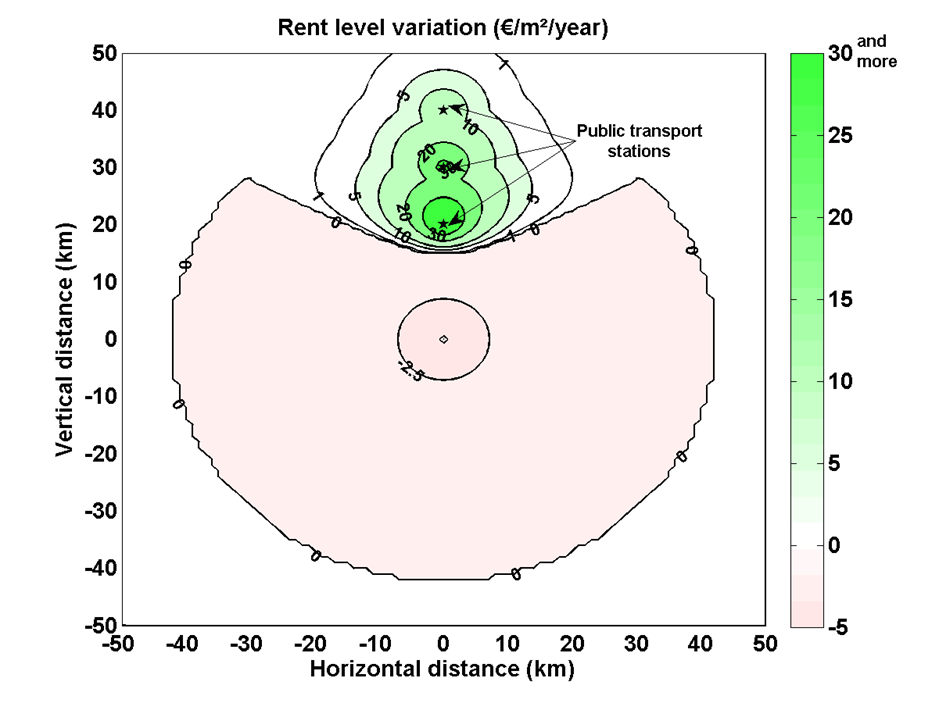
\includegraphics[width=1\columnwidth]{figures/Image3}
\par\end{centering}
\centering{}Closed city case
\end{figure}
\onslide<2> 
\begin{figure}
\begin{centering}
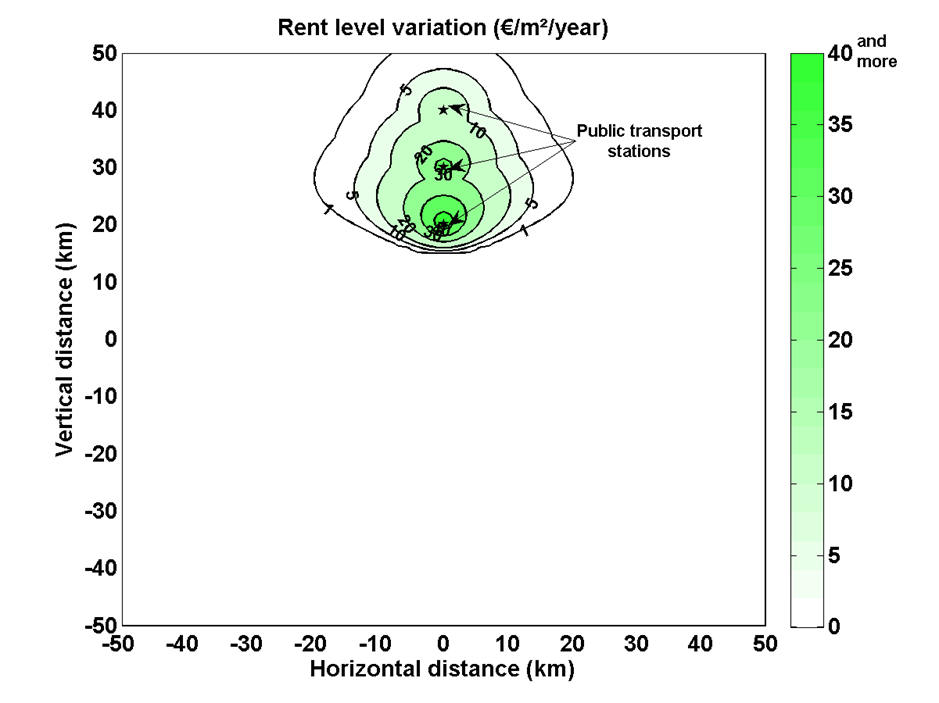
\includegraphics[width=1\columnwidth]{figures/Image6}
\par\end{centering}
\centering{}Open city case
\end{figure}
\end{overprint}

\column{3.5cm}
\begin{overprint}
\onslide<2> 

\begin{block}{}
{\small{}If transport infrastructure increases city attractiveness}{\small \par}
\end{block}
{\small{}}
%
{\small \par}\begin{block}{}
{\small{}i.e. total population increases due to transport infrastructure }{\small \par}
\end{block}
{\small{}}
%
{\small \par}\begin{block}{}
{\small{}e.g. suppose that utility in the city remains constant (\textquotedblleft open
city\textquotedblright ) }{\small \par}
\end{block}
\end{overprint}
\end{columns}

\end{frame}

\begin{frame}[t]{economic theory (2)}

\begin{block}{}

This is a block without a title

the package \textquotedbl{}tikzpicture\textquotedbl{} enables to put
a shadow around pictures
\end{block}
\begin{overprint}
\onslide<1> 
\begin{figure}
\centering
\begin{tikzpicture}   
\node[blur shadow={shadow blur steps=10},fill=white,draw] at (0,0) { 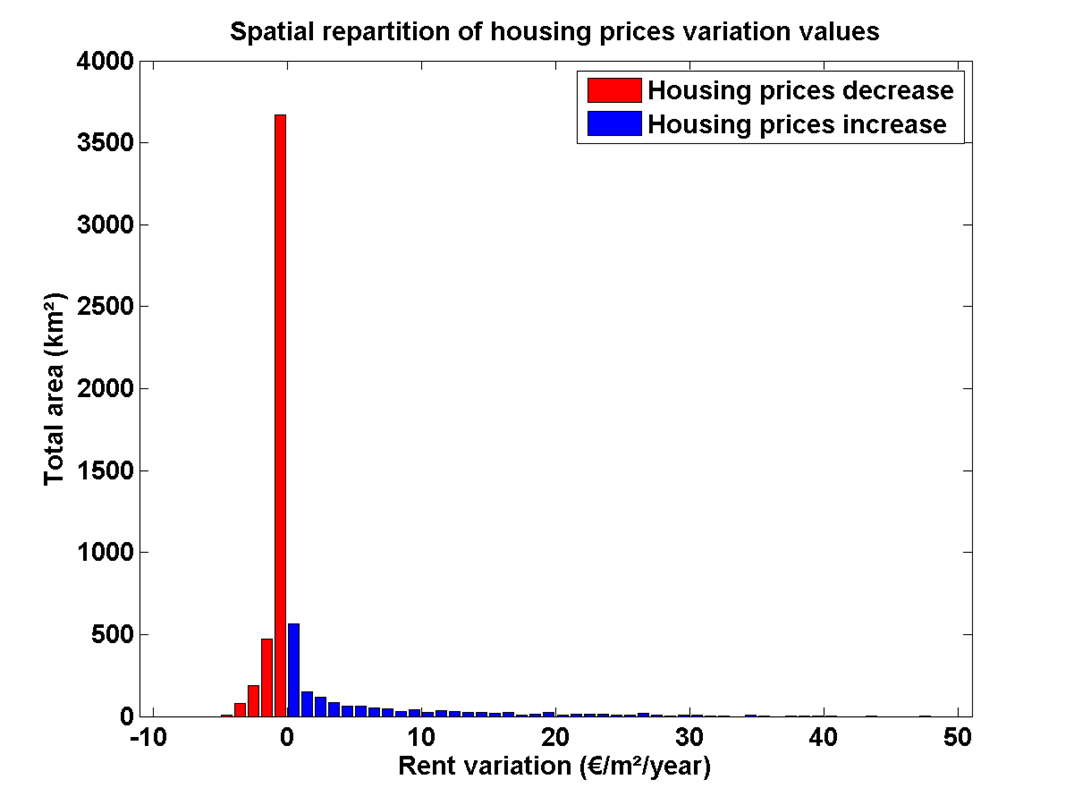
\includegraphics[height=0.5\textheight]{figures/Image4}};
\end{tikzpicture}

shadow and border around the picture
\end{figure}
\onslide<2> 
\begin{figure}
\centering
\begin{tikzpicture}   
\node[blur shadow={shadow blur steps=10},fill=white] at (0,0) { 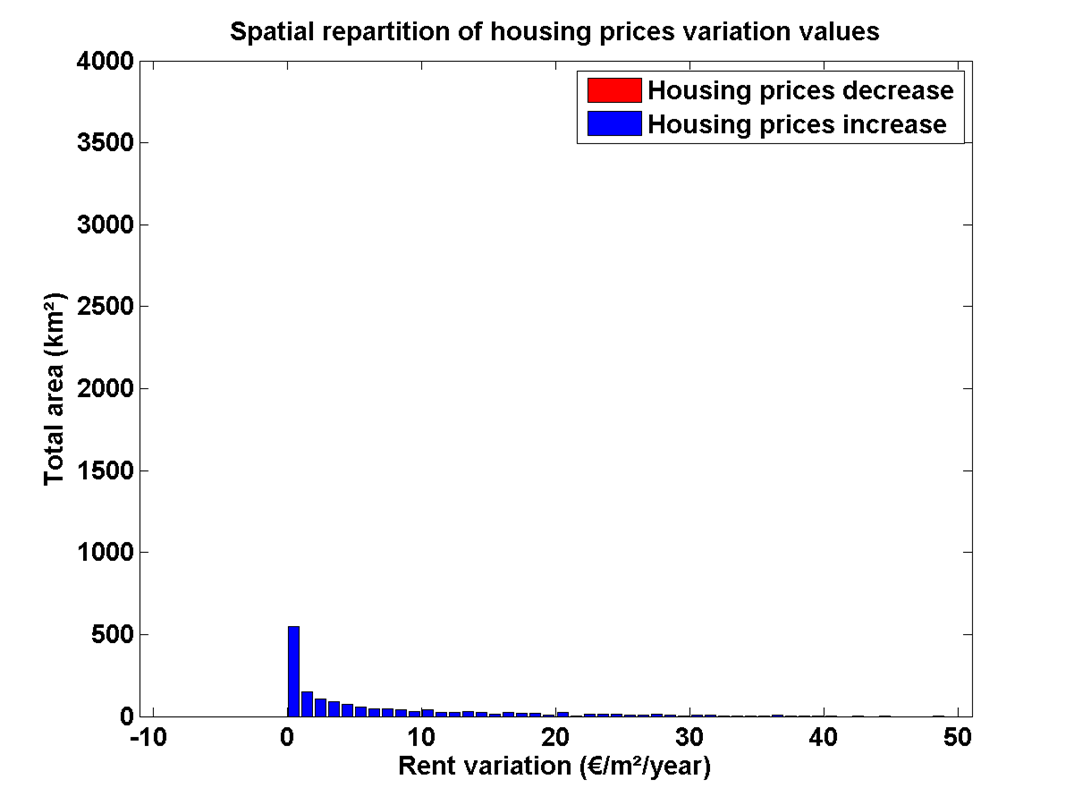
\includegraphics[height=0.5\textheight]{figures/Image7}};
\end{tikzpicture}

without the \textquotedbl{}draw\textquotedbl{}option: no border around
picture, but still the shadow
\end{figure}
\end{overprint}
\end{frame}

\begin{frame}[c]{Validation: city structure}

\begin{overprint}
\onslide<1> 

\begin{center}
\begin{figure}
\begin{centering}
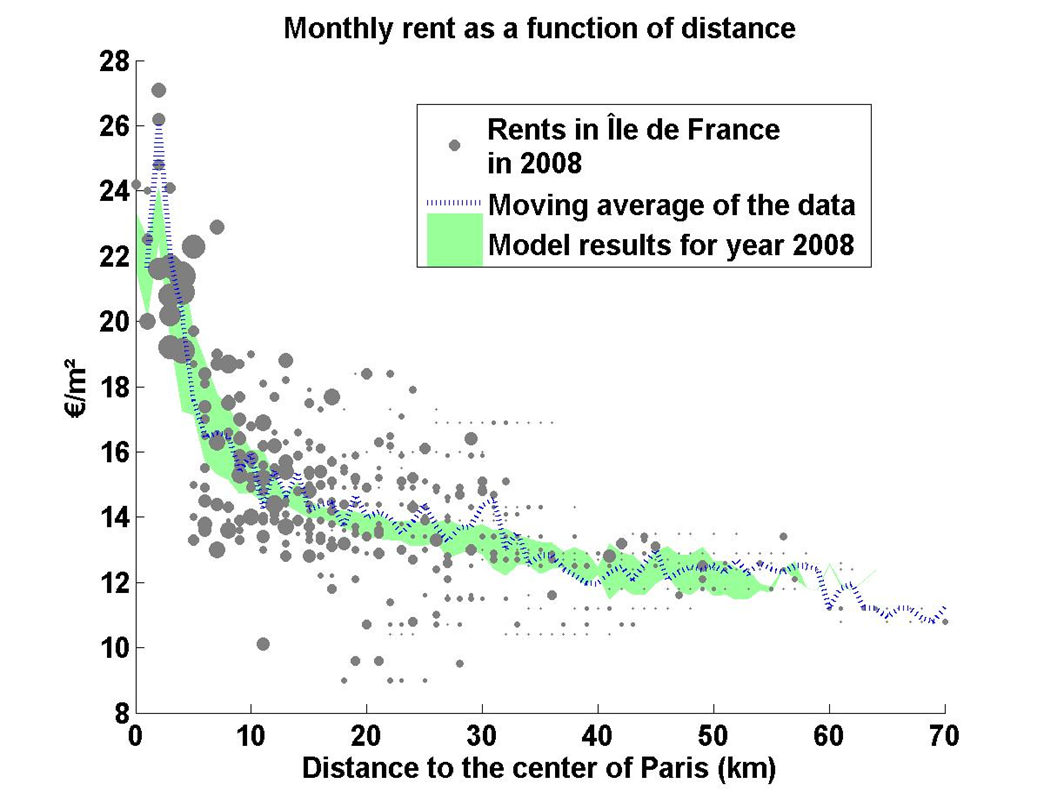
\includegraphics[width=0.7\columnwidth]{figures/loyers}
\par\end{centering}
\begin{centering}
Rents in Paris, 2008
\par\end{centering}
\centering{}$R^{2}=51.8\%$
\end{figure}
\par\end{center}
\onslide<2> 

\begin{center}
\begin{figure}
\begin{centering}
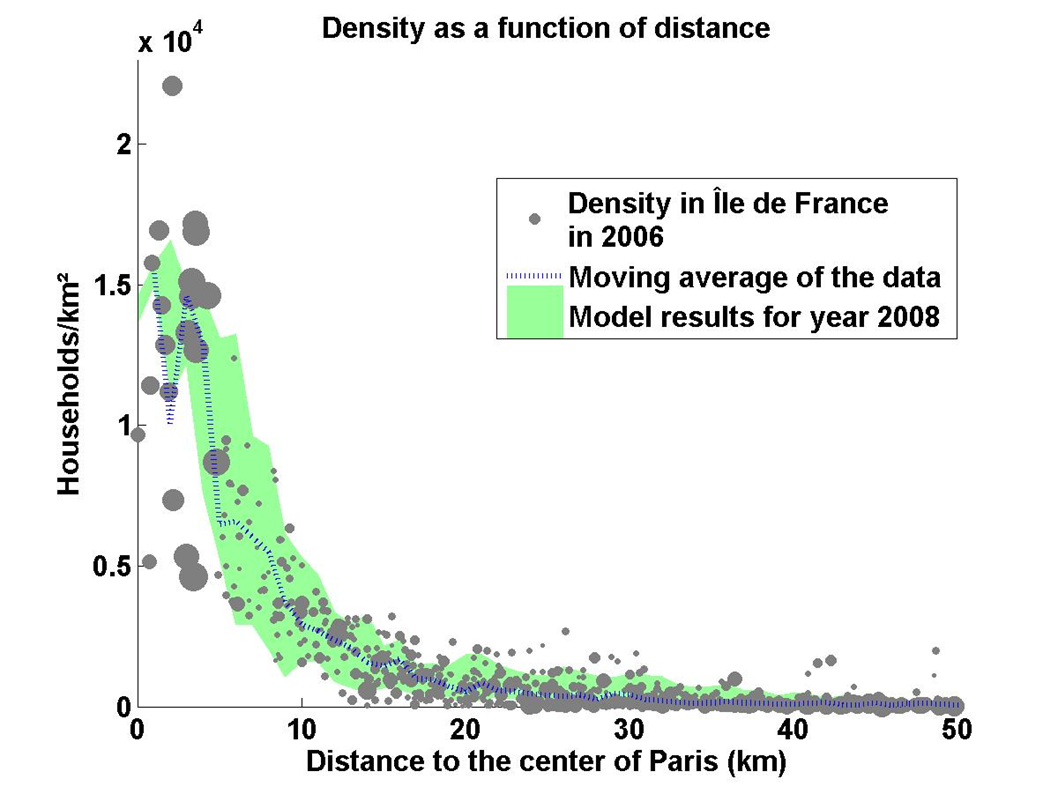
\includegraphics[width=0.7\columnwidth]{figures/density}
\par\end{centering}
\begin{centering}
Population density in Paris, 2006
\par\end{centering}
\centering{}$R^{2}=77.2\%$
\end{figure}
\par\end{center}
\end{overprint}
\end{frame}

\subsection{Basic Ideas for Proofs/Implementations}
\begin{frame}{Reduced form model }

\begin{overprint}
\onslide<1> 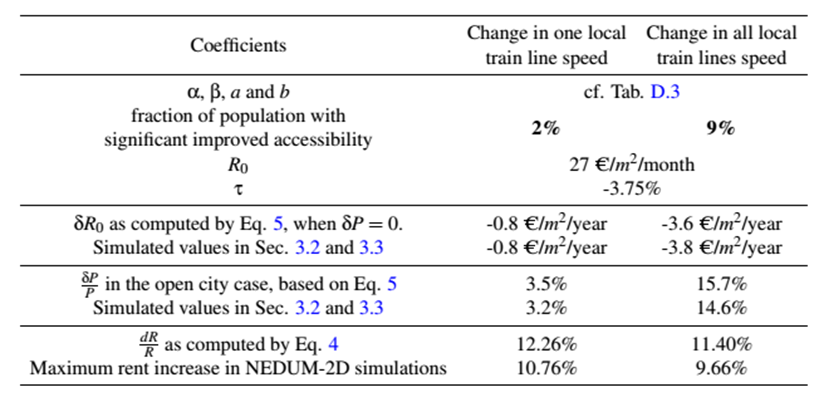
\includegraphics[width=0.95\columnwidth]{figures/table0}
\onslide<2> 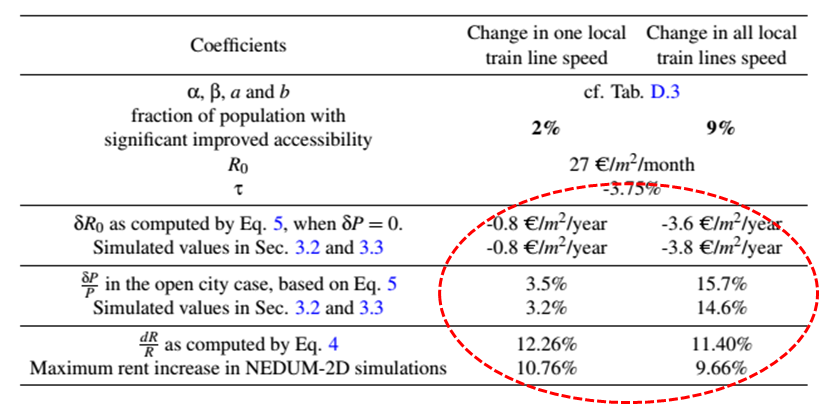
\includegraphics[width=0.95\columnwidth]{figures/table}
\end{overprint}
Less than 15\% difference between reduced-form model and simulation 
\end{frame}

\begin{frame}{Subsections}

\begin{itemize}
\item When using subsections, the dots in the outline at the top of the
page are put in different lines

\begin{itemize}
\item each line corresponds to a subsection
\end{itemize}
\item If you don't want to use subsections, you still have to indicate $\backslash subsection\{\}$
after the beginning of each section so that everything works fine
\end{itemize}
\end{frame}

\section{Conclusion}

\subsection*{}
\begin{frame}{Summary}

\begin{itemize}
\item The \alert{first main message} of your talk in one or two lines.
\item The \alert{second main message} of your talk in one or two lines.
\item Perhaps a \alert{third message}, but not more than that.
\end{itemize}
\medskip{}

\begin{itemize}
\item Outlook

\begin{itemize}
\item What we have not done yet.
\item Even more stuff.
\end{itemize}
\end{itemize}
\end{frame}

\appendix

\section*{Appendix}

\subsection*{For Further Reading}
\begin{frame}[allowframebreaks]{For Further Reading}

\beamertemplatebookbibitems
\begin{thebibliography}{1}
\bibitem{Author1990}A. Author. \newblock\emph{Handbook of Everything}.\newblock
Some Press, 1990.\beamertemplatearticlebibitems

\bibitem{Someone2002}S. Someone.\newblock On this and that\emph{.}
\newblock\emph{Journal on This and That}. 2(1):50\textendash 100,
2000.
\end{thebibliography}
\end{frame}

\end{document}
